\documentclass[a4paper,12pt,notitlepage]{article}
\usepackage{mathtools}
\usepackage{amssymb}
\usepackage{braket}
\usepackage{graphicx}
\usepackage[section]{placeins}
\title{Dynamical Systems}
\author{Richard Fox}
\date{}

\begin{document}

\begin{figure}[h]
    \centering
        \centering
        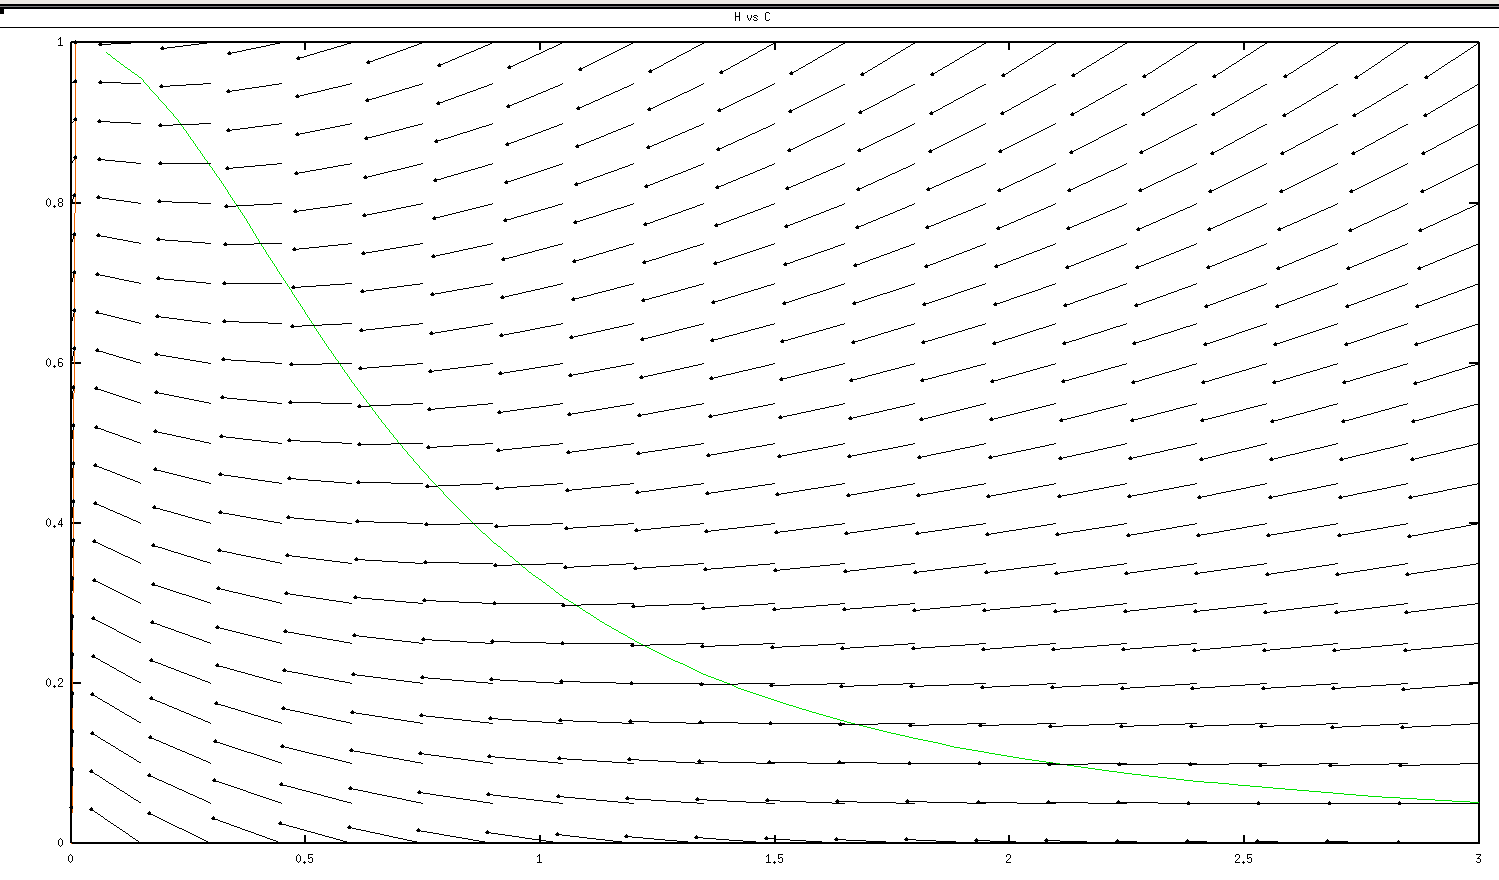
\includegraphics[width=\textwidth]{mu01.png} 
\end{figure}

\begin{figure}[h]
        \centering
        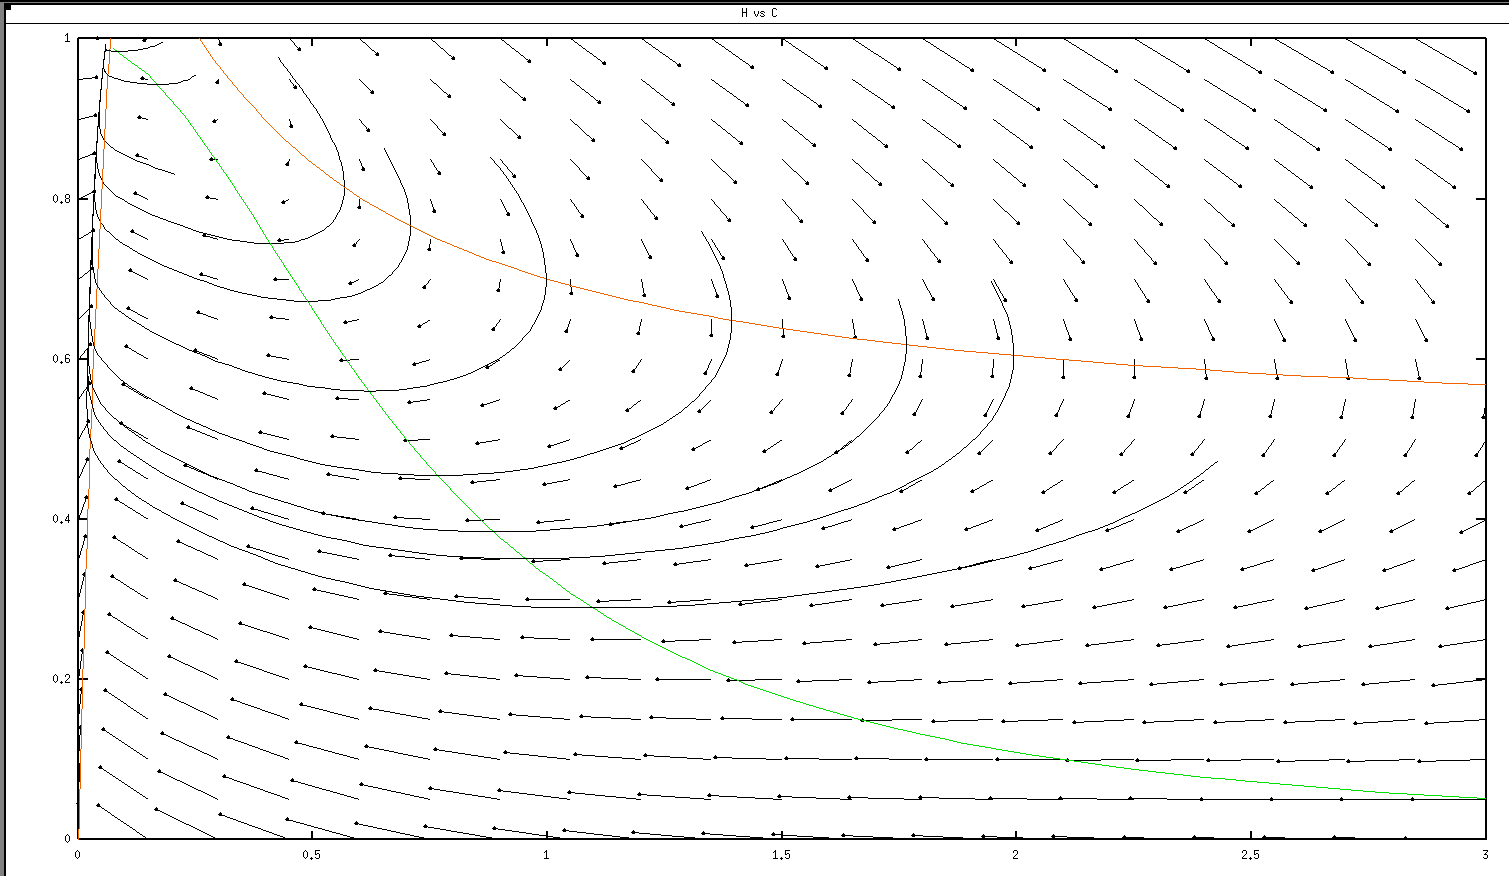
\includegraphics[width=\textwidth]{mu3.png} 
\end{figure}

\begin{figure}[h]
    \centering
        \centering
        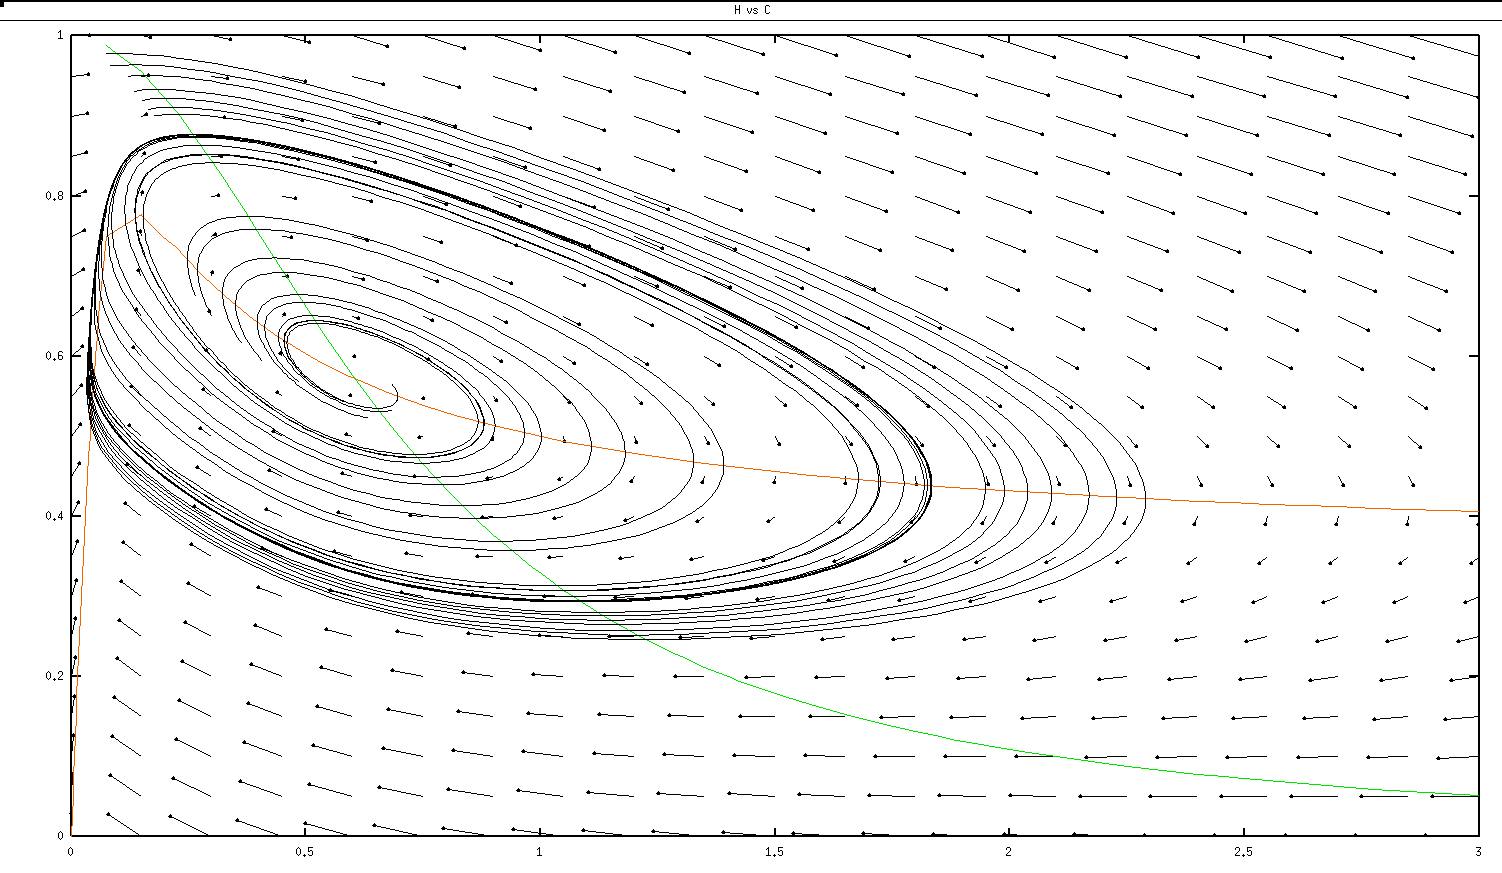
\includegraphics[width=\textwidth]{mu5.png} 
\end{figure}

\begin{figure}[h]
        \centering
        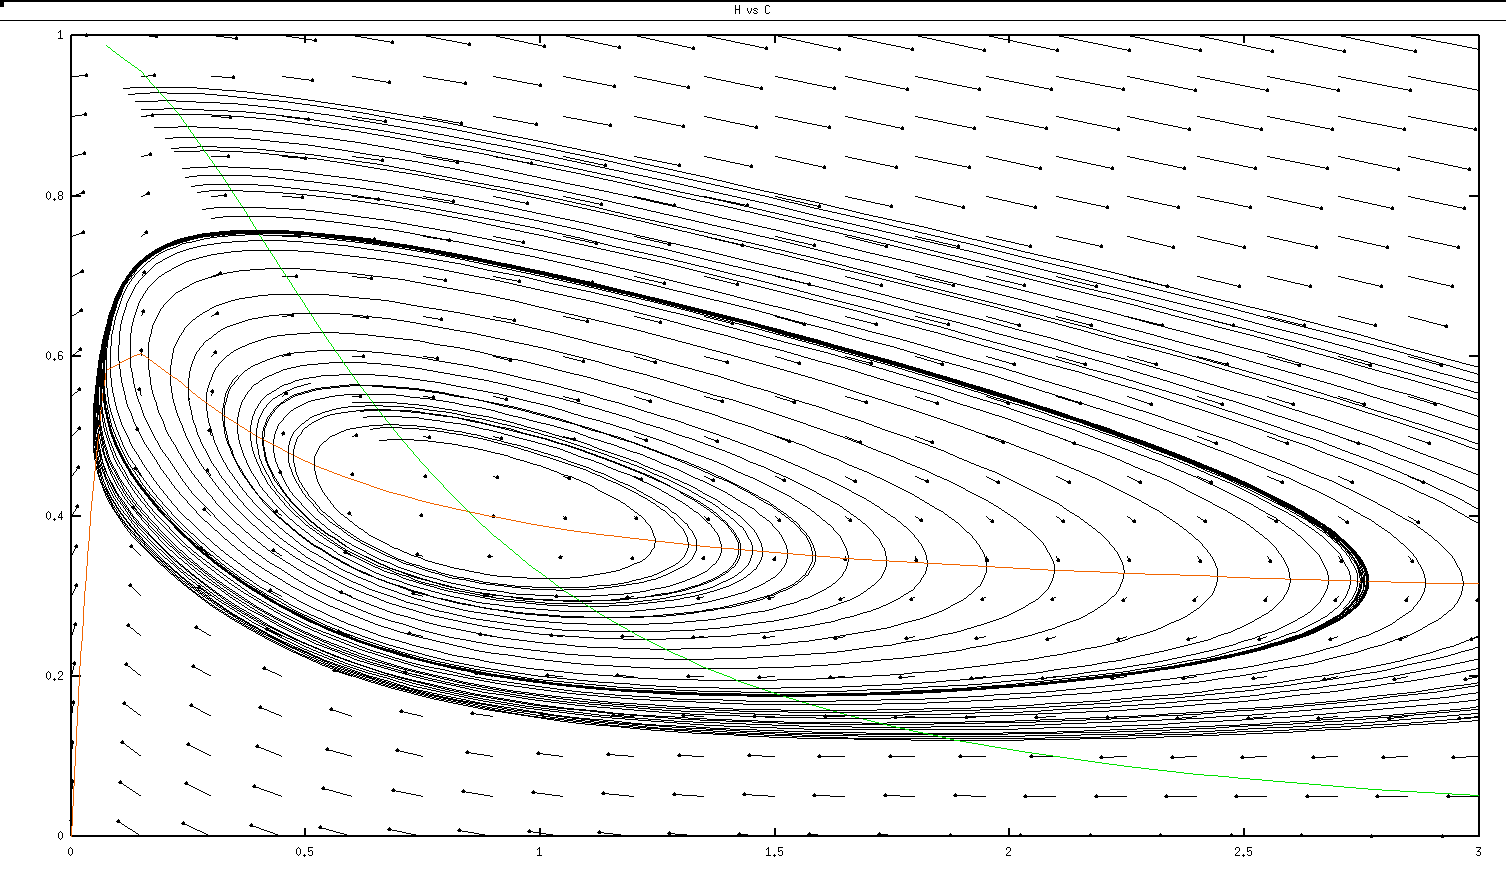
\includegraphics[width=\textwidth]{mu7.png} 
\end{figure}

\begin{figure}[h]
    \centering

        \centering
        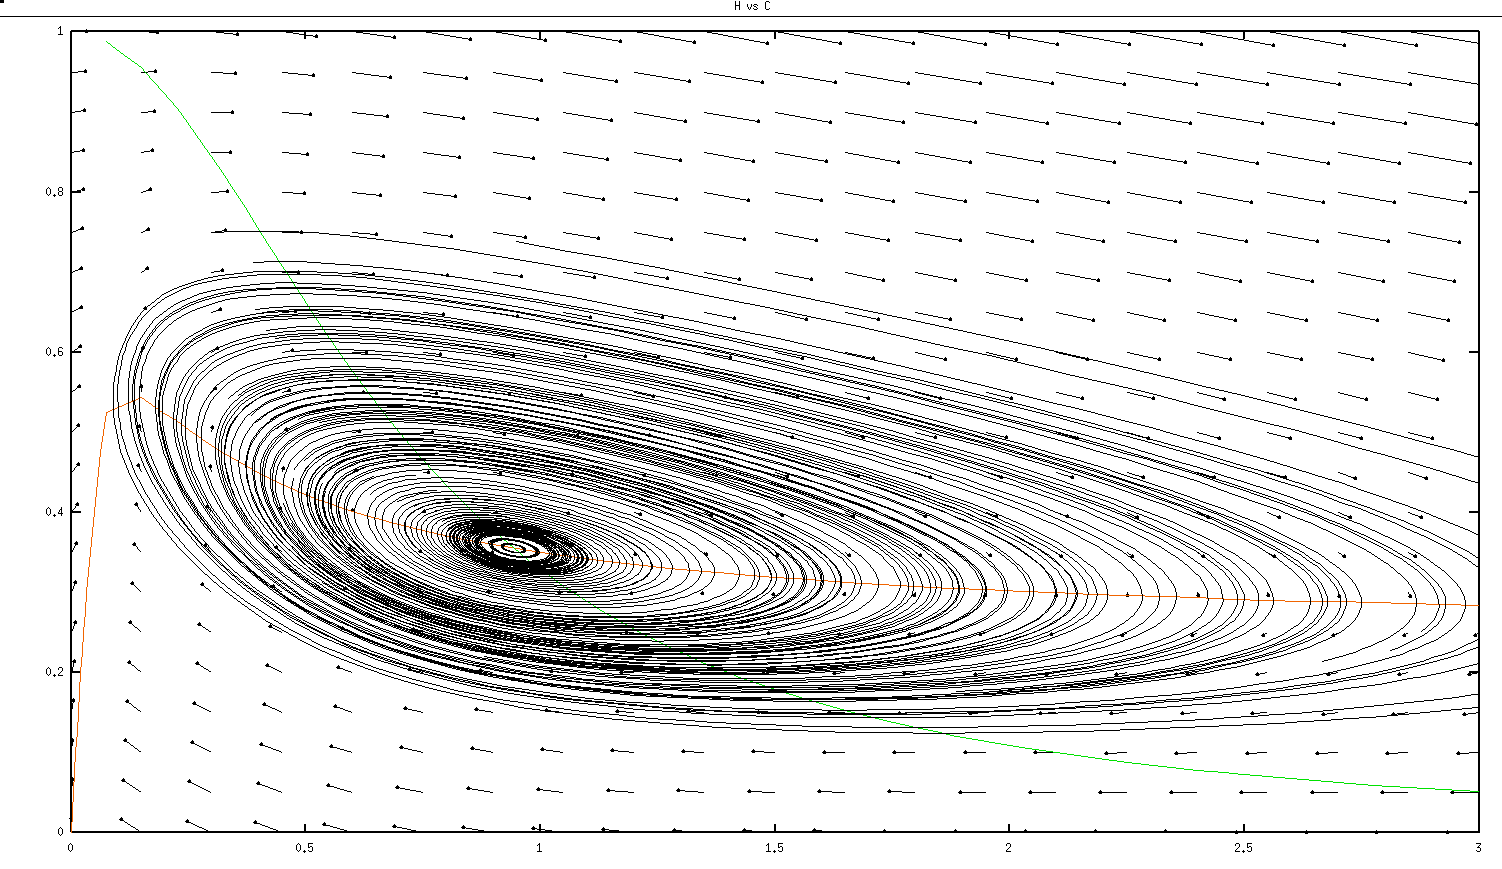
\includegraphics[width=\textwidth]{mu1.png} 
\end{figure}

\begin{figure}[h]}
        \centering
        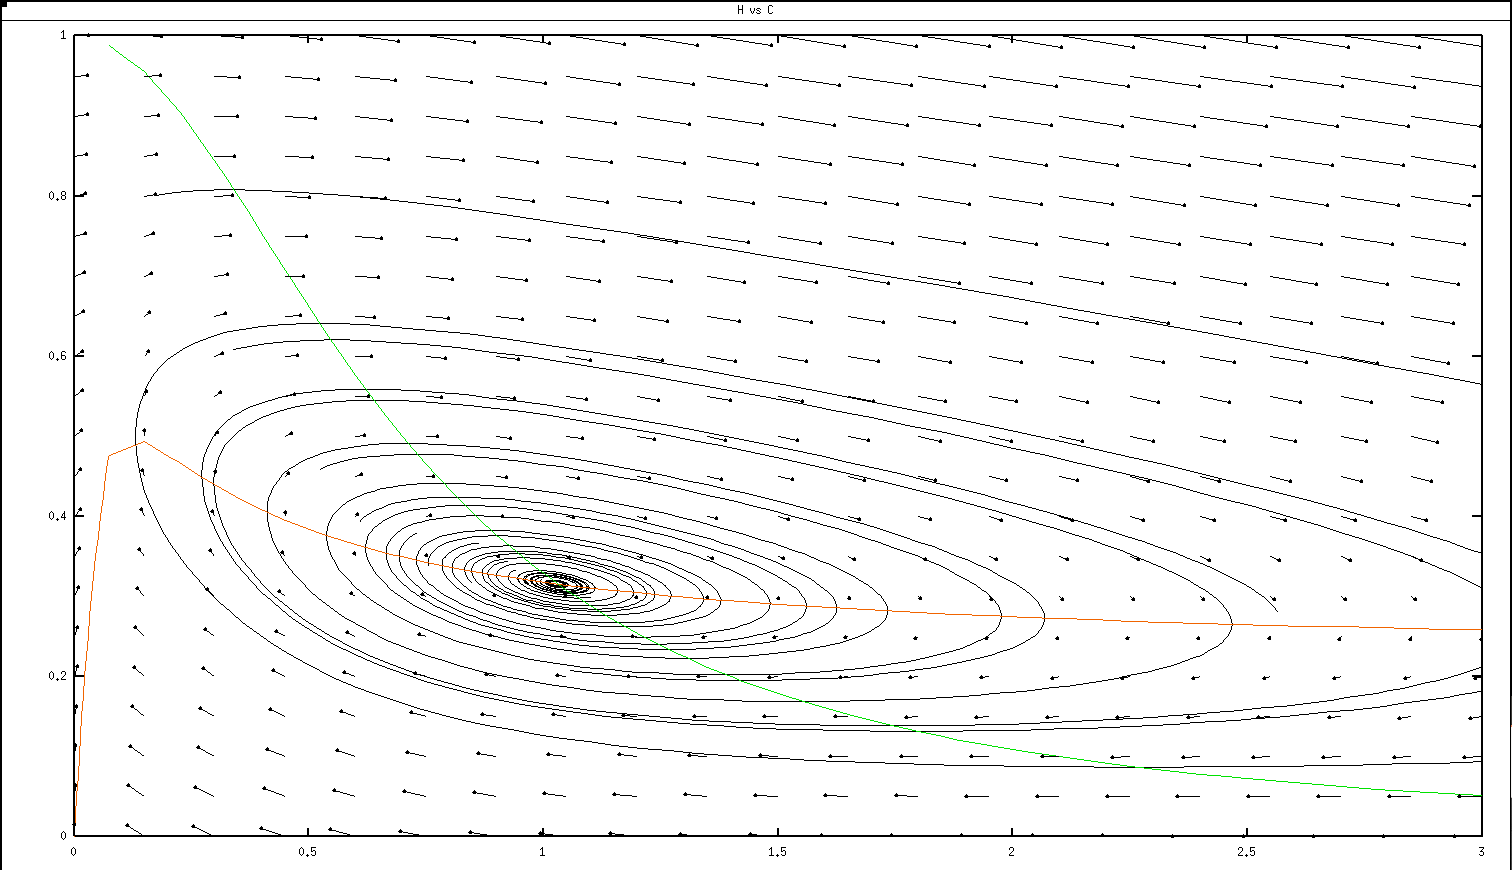
\includegraphics[width=\textwidth]{mu11.png} 
\end{figure}

\begin{figure}[h]
    \centering
        \centering
        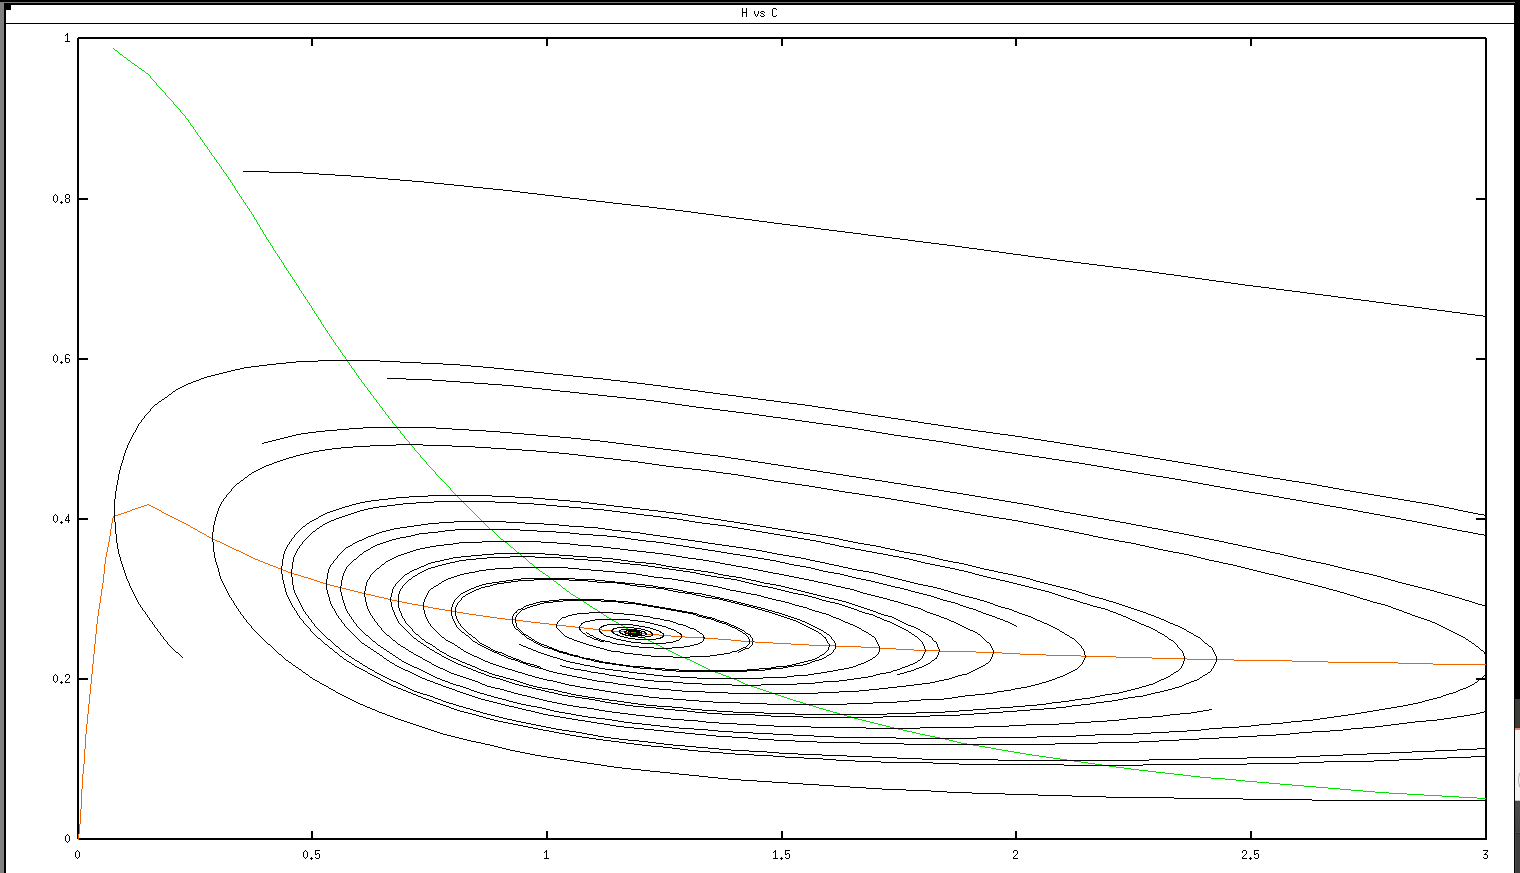
\includegraphics[width=\textwidth]{mu13.png} 
\end{figure}

\begin{figure}[h]
        \centering
        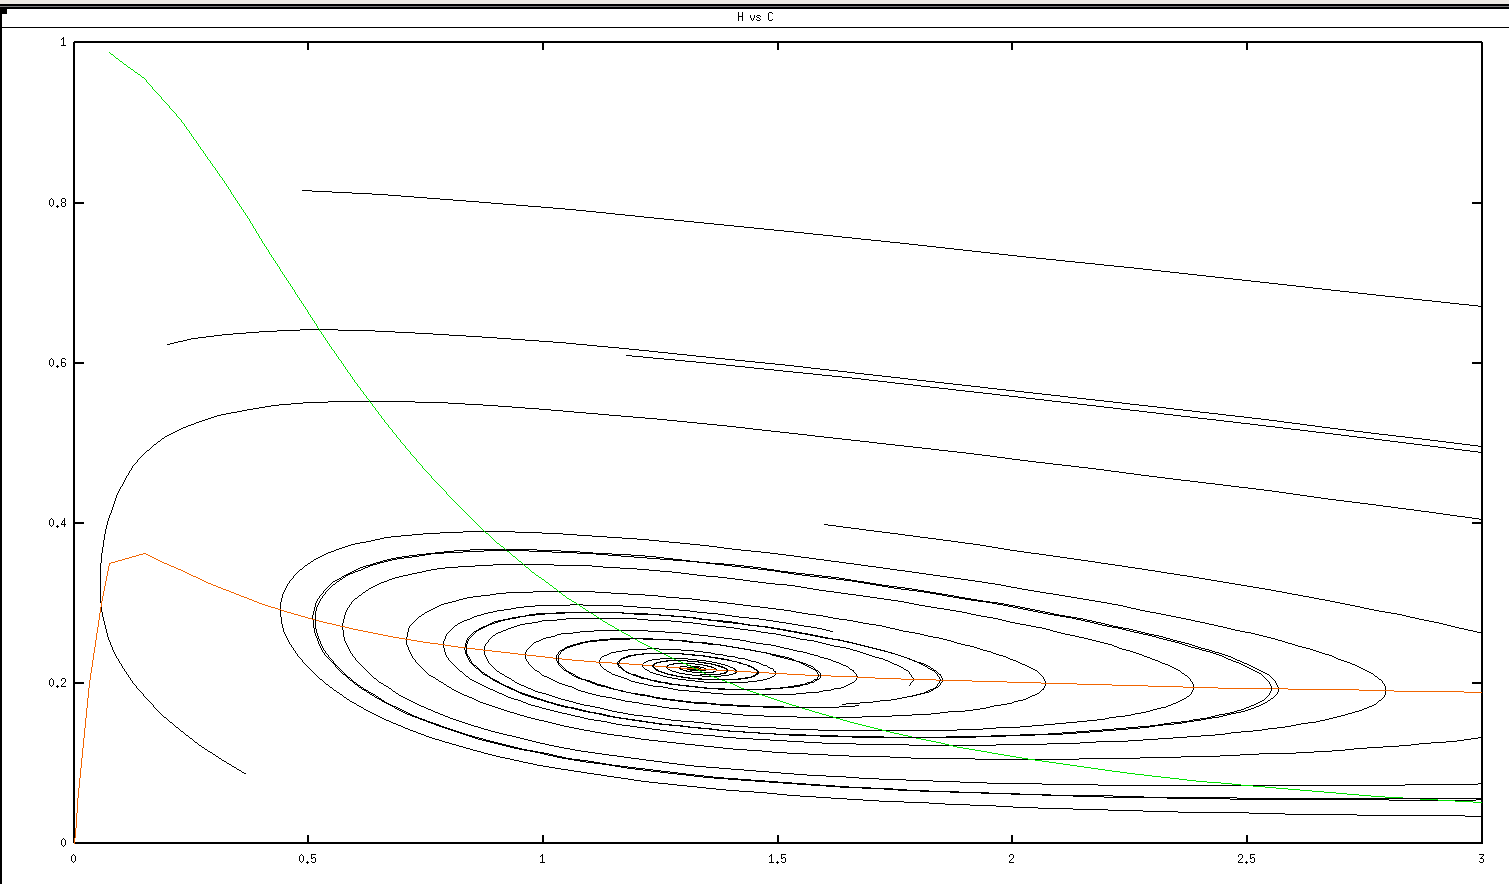
\includegraphics[width=\textwidth]{mu15.png} 
\end{figure}

\begin{figure}[h]
    \centering
        \centering
        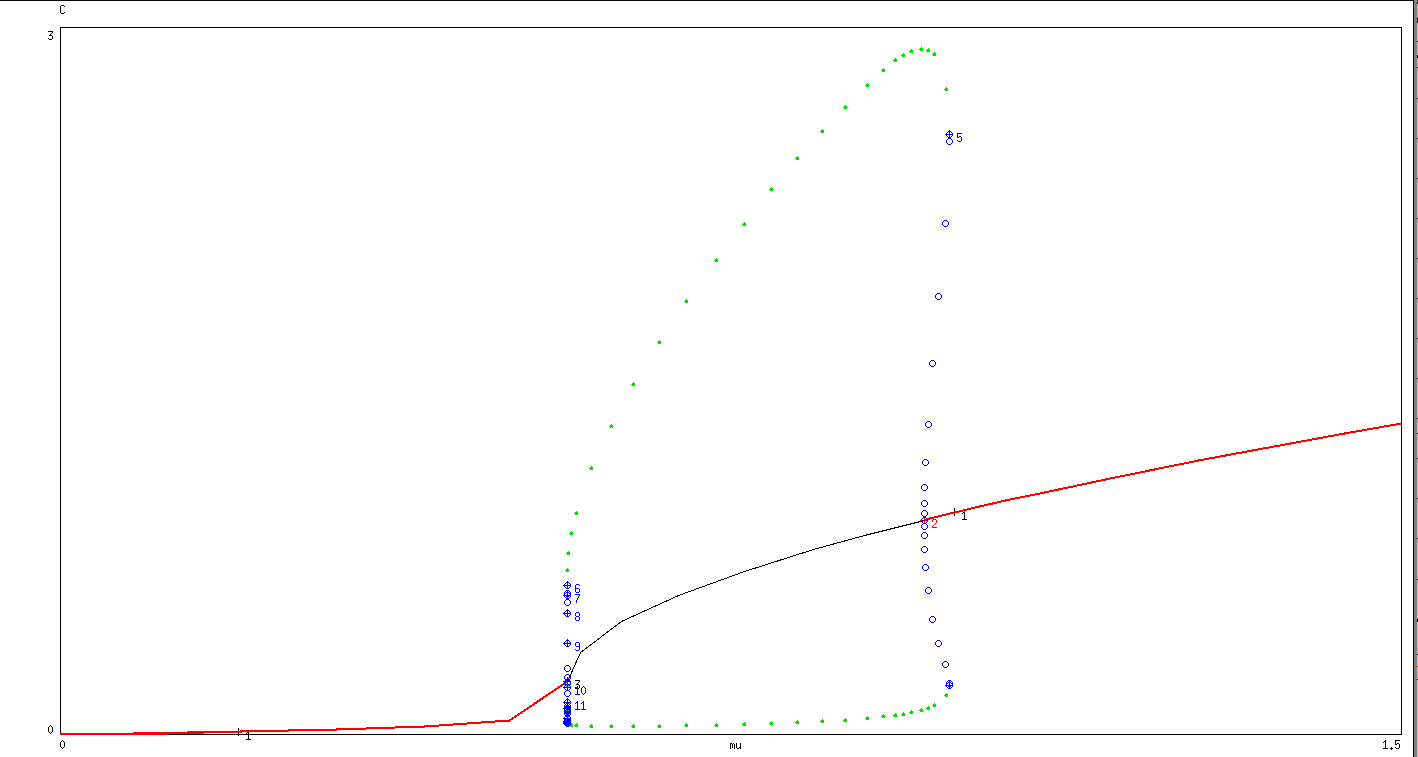
\includegraphics[width=\textwidth]{mubif.png} 
\end{figure}

\begin{figure}[h]
        \centering
        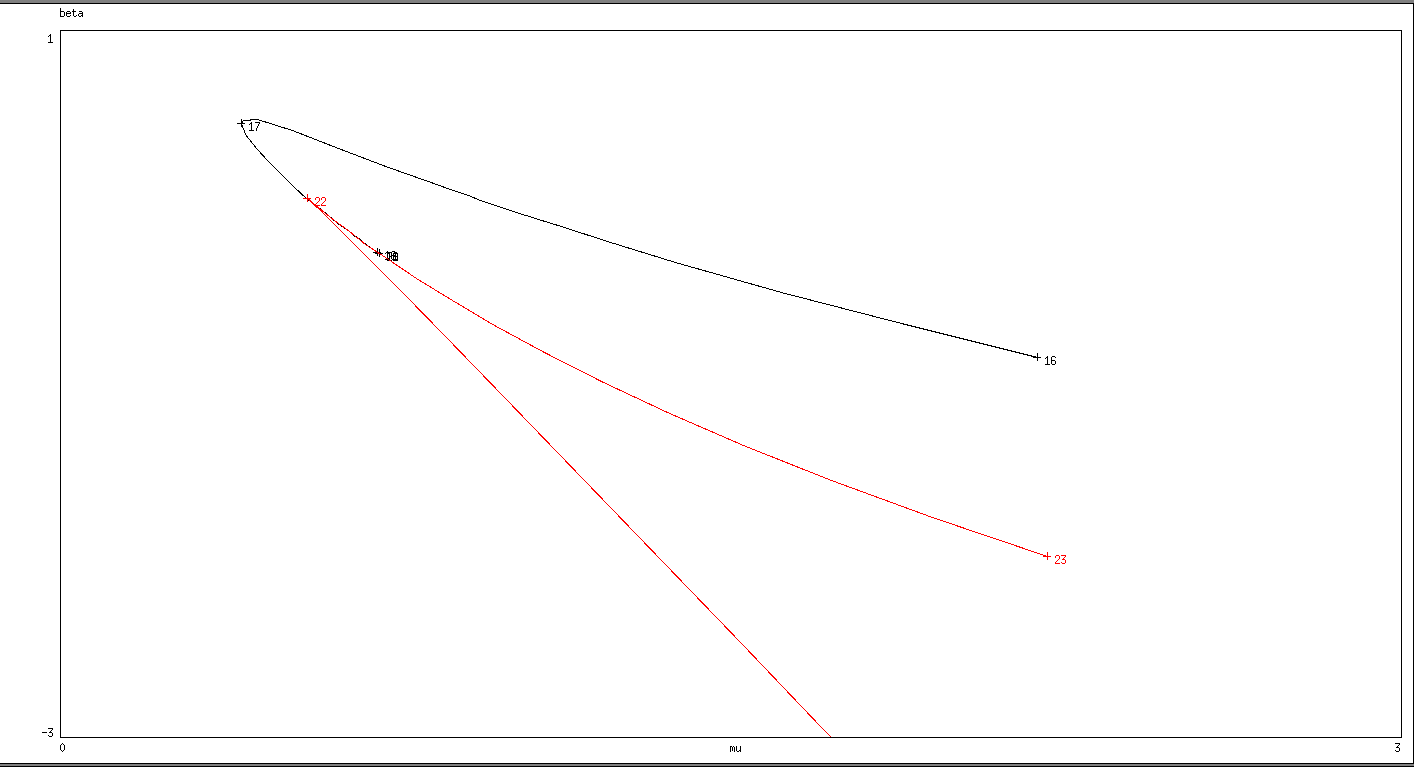
\includegraphics[width=0.9\textwidth]{2bif.png} 
\end{figure}

\begin{figure}[h]
    \centering
        \centering
        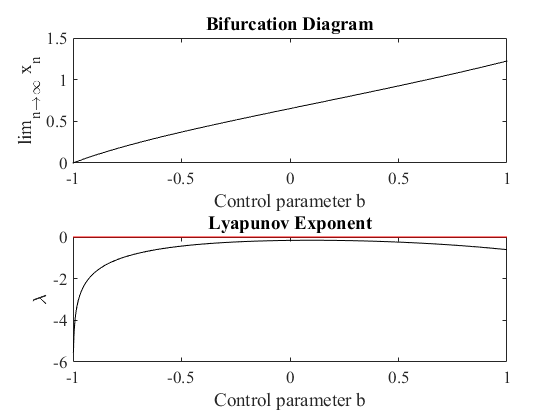
\includegraphics[width=\textwidth]{a=1.png} 

        \centering
        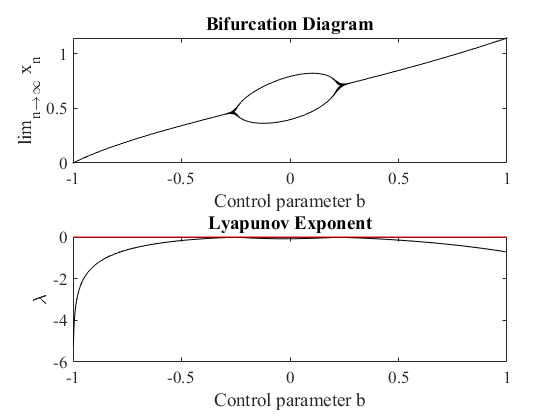
\includegraphics[width=\textwidth]{a=1_5.png} 
\end{figure}

\begin{figure}[h]
    \centering

        \centering
        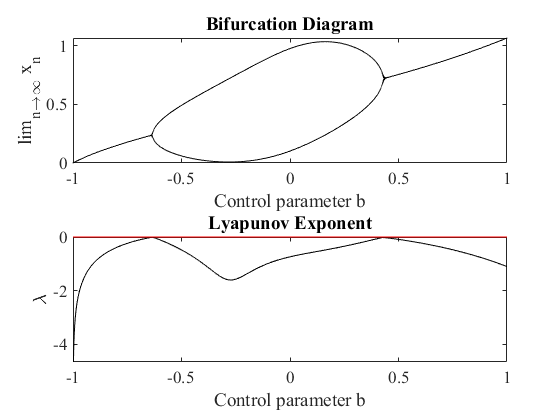
\includegraphics[width=\textwidth]{a=2.png} 

        \centering
        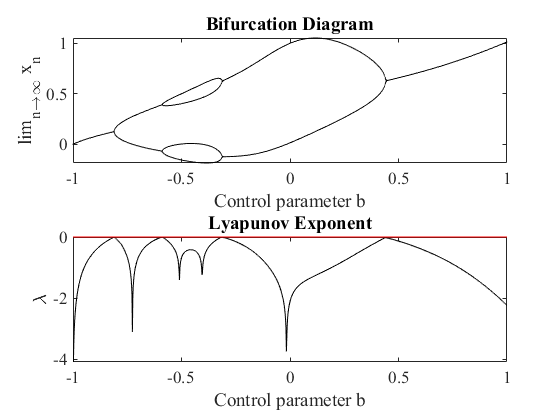
\includegraphics[width=\textwidth]{a=4.png} 
\end{figure}

\begin{figure}[h]
    \centering
        \centering
        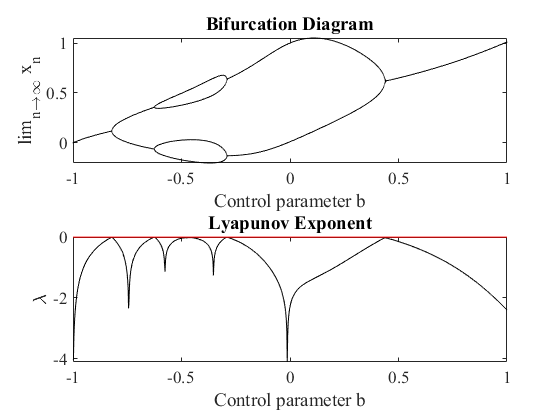
\includegraphics[width=\textwidth]{a=4_5.png} 

        \centering
        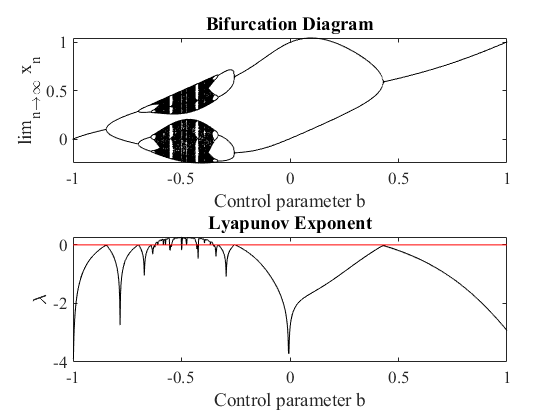
\includegraphics[width=\textwidth]{a=5.png} 
\end{figure}

\begin{figure}[h]
    \centering
        \centering
        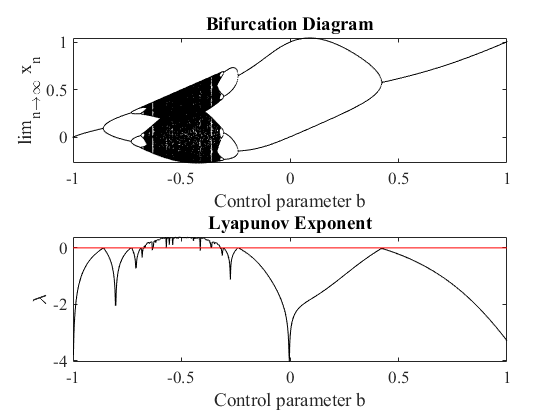
\includegraphics[width=\textwidth]{a=5_5.png} 

        \centering
        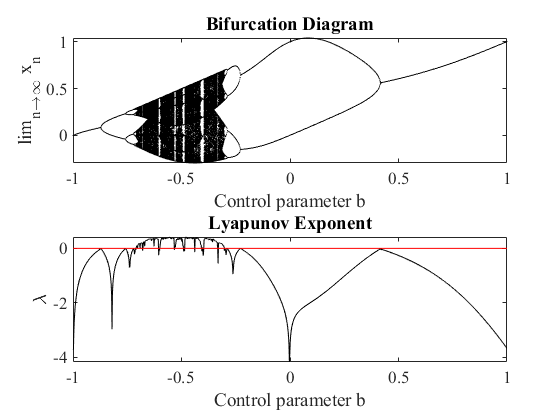
\includegraphics[width=\textwidth]{a=6.png} 
\end{figure}

\begin{figure}[h]
    \centering
        \centering
        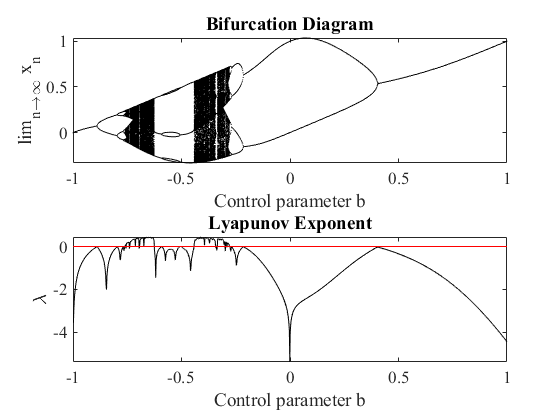
\includegraphics[width=\textwidth]{a=7.png} 

        \centering
        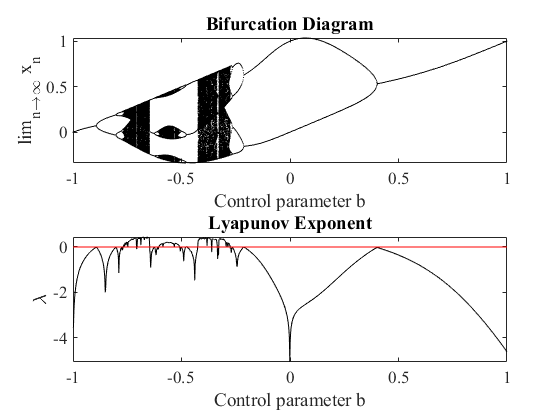
\includegraphics[width=\textwidth]{a=7_25.png} 
   
\end{figure}

\begin{figure}[h]
    \centering
        \centering
        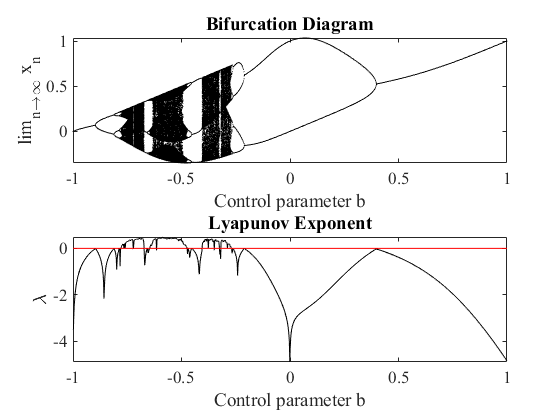
\includegraphics[width=\textwidth]{a=7_5.png} 

        \centering
        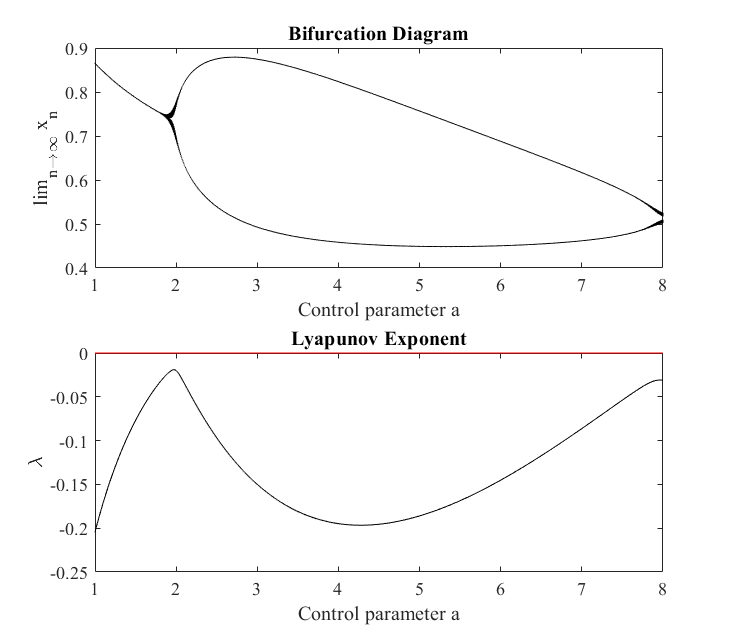
\includegraphics[width=\textwidth]{b=03921.png} 
\end{figure}

\begin{figure}[h]

        \centering
        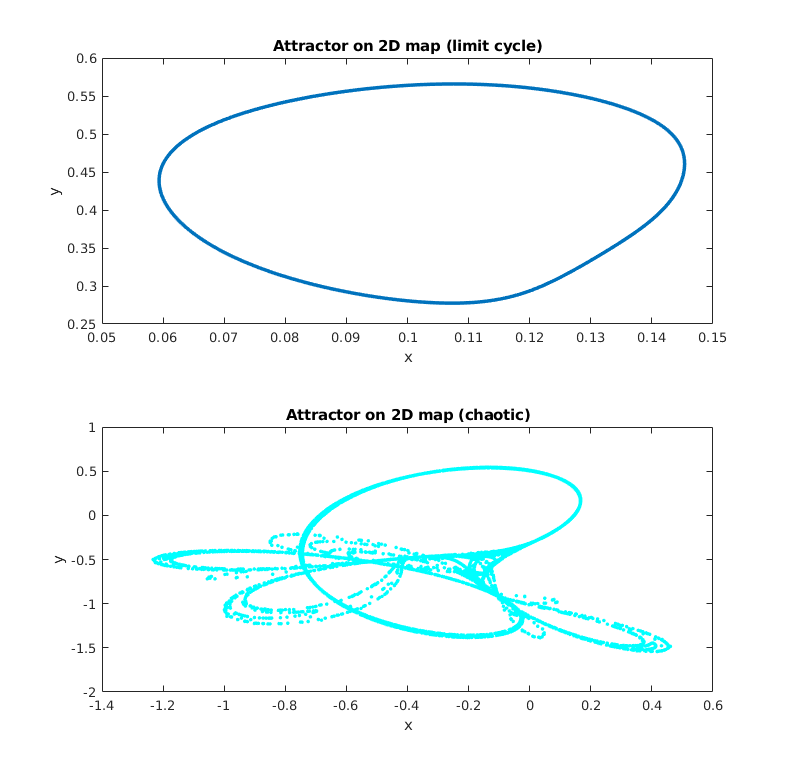
\includegraphics[width=0.9\textwidth]{Q4.png}

   

        \centering
        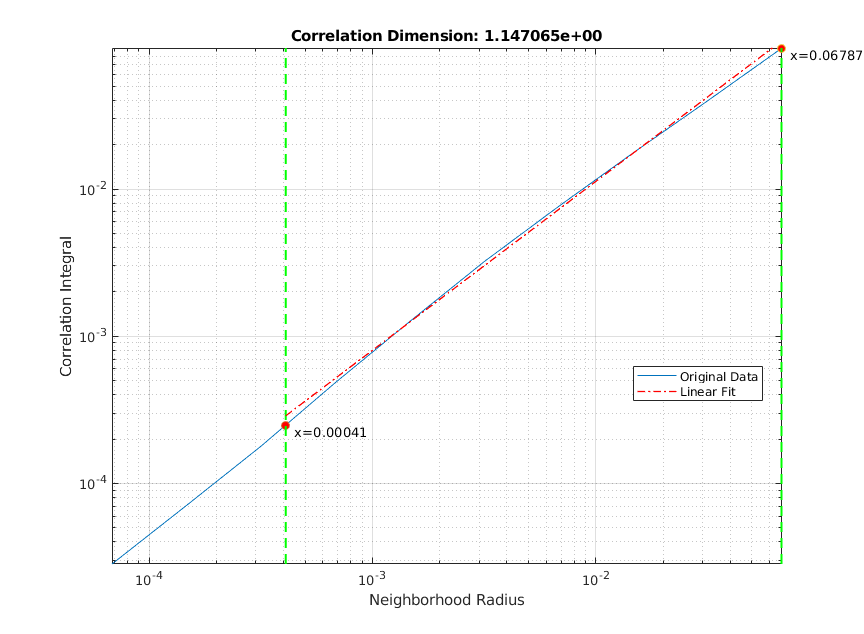
\includegraphics[width=0.9\textwidth]{CorDim.png}

\end{figure}

\end{document}